% !TEX program = xelatex
\documentclass[withoutpreface]{cumcmthesis}

\title{NIPT的时点选择与胎儿的异常判定}

\tihao{C}
\baominghao{}
\schoolname{}
\membera{}
\memberb{}
\memberc{}
\supervisor{}
\yearinput{2025}
\monthinput{9}
\dayinput{}

\graphicspath{{../results/}}

\usepackage{diagbox}
\usepackage{makecell}

\begin{document}

\maketitle

\begin{abstract}

本文围绕NIPT检测中Y染色体浓度的时间动态规律，建立浓度建模、时点优化与异常判定的分析框架。

针对问题一，267名孕妇共1082条纵向观测数据的组内相关系数ICC=0.60，提示个体聚类效应不可忽略。本文建立\textbf{广义加性混合模型（GAMM）}，以B样条基函数拟合孕周的非线性效应，引入随机截距和随机斜率刻画个体差异。模型AIC为$-$5240.80，线性混合效应模型AIC=$-$5174.04，似然比检验\textbf{$\chi^2$=76.76}（$p<10^{-15}$），RMSE=\textbf{0.0101}，非线性成分的加入带来了实质性的拟合改善。Y染色体浓度随孕周非线性上升，BMI对浓度有负向稀释作用。

针对问题二，采用\textbf{数据驱动BMI分段与双风险函数优化}确定各组最佳检测时点。以BIC准则搜索最优断点，得到BMI=30和BMI=36两个分界，将孕妇分为三组。构造风险函数$R(t)$=0.4$R_{\text{delay}}(t)$+0.6$R_{\text{inaccuracy}}(t)$，同时权衡延迟风险与检测不准确风险。优化结果为G1组（BMI$\in$[20.7,30)）最优时点\textbf{11.7周}，G2组（BMI$\in$[30,36)）\textbf{11.8周}，G3组（BMI$\in$[36,46.9)）\textbf{13.5周}，高BMI组对误差敏感性明显更高。

针对问题三，建立\textbf{多因素GAMM并结合残差分解与Monte Carlo误差传播}分析扩展因素的影响。体重与BMI的共线性严重（VIF=351），残差分解后VIF降至\textbf{1.01}。检验发现年龄（$p$=0.309）和体重残差（$p$=0.685）均不显著，BMI单因素已足够。将孕妇细分为4组后最优时点分别为12.8、13.3、13.3、24.8周，500次MC模拟显示高BMI组95\%置信区间为[11.0,24.6]周，样本量不足是时点估计波动大的主要原因。

针对问题四，女性胎儿缺乏Y染色体标记，本文转而建立基于\textbf{多元马氏距离的异常检测方法}，选取Z13、Z18、Z21、ZX、BMI、X浓度共6维特征构建异常评分。该方法AUC=\textbf{0.574}，优于基线Z值阈值法（AUC=0.492），在第85百分位阈值处取得最佳F1=0.217，召回率26.9\%。检测能力受限于异常与正常样本在特征空间中的高度重叠。

本文的创新点在于，（1）GAMM捕捉孕周非线性效应，似然比检验量化改进幅度（$\chi^2$=76.76）；（2）双风险函数将NIPT时点选择转化为可优化的决策问题，定量权衡延迟风险与准确性风险；（3）残差分解消除体重与BMI共线性（VIF从351降至1.01），MC模拟量化高BMI组时点不确定性。

\end{abstract}

\keywords{NIPT检测；广义加性混合模型（GAMM）；BMI分段优化；Monte Carlo误差传播；马氏距离异常检测}


\section{问题重述}

无创产前检测（NIPT）通过分析孕妇外周血中的游离胎儿DNA片段来评估胎儿的遗传状态。当胎儿为男性时，母体血液中可检测到Y染色体特异性序列，其浓度随孕周增长而升高。孕妇的体质量指数（BMI）越高，母体自身游离DNA对胎儿DNA的稀释效应越强，导致检测信噪比下降。

本文围绕以下四个问题展开建模。问题一要求建立Y染色体浓度关于孕周与BMI的定量模型，刻画浓度随孕周的非线性增长趋势及BMI的稀释作用。问题二要求按BMI水平对孕妇分组，在每组内确定NIPT的最优检测时点，使检测的准确性与时效性达到综合最优。问题三将模型扩展至包含年龄、体重、身高等多因素，评估不同体征组合下的检测达标率，并分析测量误差在模型中的传播效应。问题四针对女性胎儿（无Y染色体信号），利用Z值等指标建立染色体非整倍体异常的判别模型。


\section{问题分析}

\subsection{问题一分析}

附件数据包含267名孕妇共1082次纵向检测记录，每名孕妇平均约4次观测，构成非平衡面板结构。同一孕妇的重复测量之间存在显著相关性（组内相关系数ICC约0.60），若使用普通最小二乘回归将低估标准误并产生虚假显著性。Y染色体浓度随孕周的变化呈非线性特征，BMI的稀释效应可能与孕周存在交互作用。因此需要采用能同时处理个体聚类效应和非线性趋势的纵向数据模型。

\subsection{问题二分析}

检测时点的选择面临双重约束。过早检测时胎儿DNA浓度偏低，检测灵敏度不足；过晚检测则压缩了后续临床干预的时间窗口。不同BMI组别的孕妇DNA浓度曲线形态和达标时间存在系统性差异，需要在分组基础上构建同时反映准确性风险和延迟风险的目标函数，通过优化求解各组的最优时点。

\subsection{问题三分析}

引入年龄、体重、身高等多因素后，模型维度增加，变量间可能存在共线性（如体重与BMI高度相关）。达标率的评估需要在多维体征空间上进行条件概率计算。测量误差从自变量端传入模型后，会通过非线性映射放大或缩小，需利用Delta方法或蒙特卡洛模拟量化其对预测结果的影响。

\subsection{问题四分析}

女性胎儿缺乏Y染色体标记，无法直接复用前三问的浓度模型。染色体非整倍体的检测依赖对全基因组测序覆盖度的统计比较，Z值衡量目标染色体读数相对参考分布的偏离程度。正常与异常样本的Z值分布存在重叠区域，单一阈值难以兼顾灵敏度与特异度，需要结合多个指标构建综合判别规则，并通过ROC分析评价分类性能。


\section{模型假设}

\begin{enumerate}
    \item 同一孕妇不同时间点的检测样本彼此独立（给定个体随机效应后）。
    \item 孕妇个体差异可用随机截距和随机斜率充分刻画。
    \item Y染色体浓度的测量误差服从零均值正态分布。
    \item 孕妇BMI在整个孕期检测窗口内近似不变。
    \item 胎儿DNA释放速率与孕妇体征之间不存在未观测的混杂因素。
    \item 染色体非整倍体异常的表现独立于检测时间点。
\end{enumerate}


\section{符号说明}

\begin{table}[H]
\centering
\begin{tabular}{clc}
\toprule
符号 & 说明 & 单位 \\
\midrule
$y_{ij}$ & 第$i$名孕妇第$j$次检测的Y染色体浓度 & 比例值 \\
$t_{ij}$ & 第$i$名孕妇第$j$次检测的孕周 & 周 \\
$\mathrm{BMI}_i$ & 第$i$名孕妇的体质量指数 & kg/m$^2$ \\
$b_{0i},\, b_{1i}$ & 第$i$名孕妇的随机截距与随机斜率 & -- \\
$s(\cdot)$ & B样条基函数 & -- \\
$R(t)$ & NIPT检测总风险函数 & -- \\
$R_{\text{delay}}(t)$ & 延迟风险分量 & -- \\
$R_{\text{inacc}}(t)$ & 不准确风险分量 & -- \\
$T^*$ & 最优NIPT检测时点 & 周 \\
$P(y \geq c \mid t, g)$ & BMI组$g$在孕周$t$的达标比例 & -- \\
$d_M(\mathbf{x})$ & 马氏距离 & -- \\
$\sigma_\varepsilon$ & 残差标准差 & -- \\
$N$ & 样本量 & -- \\
\bottomrule
\end{tabular}
\end{table}


\section{问题一的建立与求解}

267名孕妇共1082条纵向观测数据中，每名孕妇平均包含约4个时间点的重复测量，个体内相关性对参数估计有直接影响，需要在建模中加以处理。

\subsection{混合模型框架的选择依据}

为评估个体层面聚类效应的强度，首先计算组内相关系数（ICC）。以$\sigma^2_b$表示个体间方差、$\sigma^2_\varepsilon$表示残差方差，ICC定义为
\begin{equation}
  \mathrm{ICC} = \frac{\sigma^2_b}{\sigma^2_b + \sigma^2_\varepsilon}
\end{equation}

计算结果为$\mathrm{ICC}=0.60$，Y染色体浓度总变异的60\%来源于个体间差异。若采用合并OLS回归忽略这一聚类结构，标准误将被系统性低估，假阳性膨胀。混合模型框架通过随机效应显式建模个体异质性，可保证纵向重复测量下统计推断的有效性。

\subsection{广义加性混合模型的建立}

探索性分析表明，Y染色体浓度随孕周的变化呈非线性趋势，线性假设拟合不足。本文建立\textbf{广义加性混合模型（GAMM，记为M1）}作为主模型，同时建立\textbf{线性混合效应模型（LME，记为M2）}作为基准，通过嵌套比较评估非线性成分的贡献。

GAMM模型（M1）的具体形式为
\begin{equation}\label{eq:gamm}
  y_{ij} = \beta_0 + s_1(t_{ij}) + s_2(\mathrm{BMI}_i) + b_{0i} + b_{1i}\,t_{ij} + \varepsilon_{ij}
\end{equation}

其中$y_{ij}$为第$i$名孕妇在第$j$次观测时的Y染色体浓度，$t_{ij}$为对应孕周。各成分含义如下。

\begin{itemize}
  \item $s_1(\cdot)$为孕周的非线性平滑函数，采用B样条基函数，自由度$\mathrm{df}=4$；
  \item $s_2(\cdot)$为BMI的非线性平滑函数，采用B样条基函数，自由度$\mathrm{df}=3$；
  \item $b_{0i} \sim N(0,\,\sigma^2_{b0})$为随机截距，刻画个体基线浓度差异；
  \item $b_{1i} \sim N(0,\,\sigma^2_{b1})$为孕周的随机斜率，刻画个体浓度增长速率差异；
  \item $\varepsilon_{ij} \sim N(0,\,\sigma^2_\varepsilon)$为观测误差。
\end{itemize}

LME基准模型（M2）将两个平滑函数替换为线性项
\begin{equation}\label{eq:lme}
  y_{ij} = \beta_0 + \beta_1\,t_{ij} + \beta_2\,\mathrm{BMI}_i + b_{0i} + b_{1i}\,t_{ij} + \varepsilon_{ij}
\end{equation}

M2与M1共享相同的随机效应结构，二者构成嵌套关系，可通过似然比检验直接比较。

\subsubsection{模型求解步骤}

模型估计按以下步骤执行。

\textbf{Step 1}（数据预处理）\quad 对267名孕妇的1082条观测记录进行缺失值检查与异常值筛查，确认数据完整性后按孕妇编号排列，以适配混合模型的分组结构。

\textbf{Step 2}（参数估计）\quad 采用限制最大似然法（REML）估计方差成分，固定效应参数通过L-BFGS优化器求解。REML在方差分量估计上具有无偏性，适合样本量有限的纵向数据。

\textbf{Step 3}（模型比较）\quad 对M1和M2分别以ML重新拟合（保证似然比检验的有效性），计算似然比统计量$\Lambda = 2(\ell_{\mathrm{M1}} - \ell_{\mathrm{M2}})$，在$\chi^2$分布下检验非线性成分的显著性。

\textbf{Step 4}（残差诊断）\quad 对最优模型的残差进行正态性检验（Shapiro-Wilk）和分布形态分析（偏度、峰度），验证模型假设的合理性。

\subsection{模型求解结果}

表~\ref{tab:q1-compare}汇总了M1（GAMM）与M2（LME）在主要评价指标上的对比结果。

\begin{table}[H]
  \centering
  \caption{GAMM（M1）与LME（M2）模型评价指标对比}\label{tab:q1-compare}
  \begin{tabular}{lcccc}
    \toprule
    模型 & AIC & BIC & RMSE & 对数似然 \\
    \midrule
    M1（GAMM） & $-5240.80$ & $-5180.96$ & 0.0101 & 2632.40 \\
    M2（LME）  & $-5174.04$ & $-5139.13$ & 0.0111 & --- \\
    \bottomrule
  \end{tabular}
\end{table}

似然比检验结果为$\chi^2=76.76$（$\mathrm{df}=5$，$p<10^{-15}$），M1在统计意义上优于M2。M1的AIC较M2低66.76，BIC低41.83，RMSE降低约9\%，三项指标一致支持非线性模型。

M1的固定效应估计如下。截距$\hat{\beta}_0=0.0107$；孕周B样条基系数依次为$0.0153$、$0.0173$、$0.0434$、$0.1238$，呈递增趋势，反映Y染色体浓度随孕周加速上升；BMI的B样条基系数为$0.1023$、$0.0127$、$0.0150$。随机效应方面，随机截距方差$\hat{\sigma}^2_{b0}=0.001886$，随机斜率方差$\hat{\sigma}^2_{b1}=0.000008$，个体基线差异远大于斜率差异，与ICC=0.60的结果一致。

残差诊断显示偏度为$0.125$，峰度为$4.15$，Shapiro-Wilk统计量$W=0.943$。残差分布接近对称，峰度略高于正态分布的理论值3，存在轻微尖峰，但在$n=1082$的样本量下对REML估计的稳健性影响有限。

图~\ref{fig:q1-partial}展示了M1与M2在孕周和BMI两个维度上的偏效应对比。GAMM的孕周偏效应曲线呈非线性上升形态，孕晚期阶段斜率增大明显，LME仅能以固定斜率的直线近似这一趋势。

\begin{figure}[H]
  \centering
  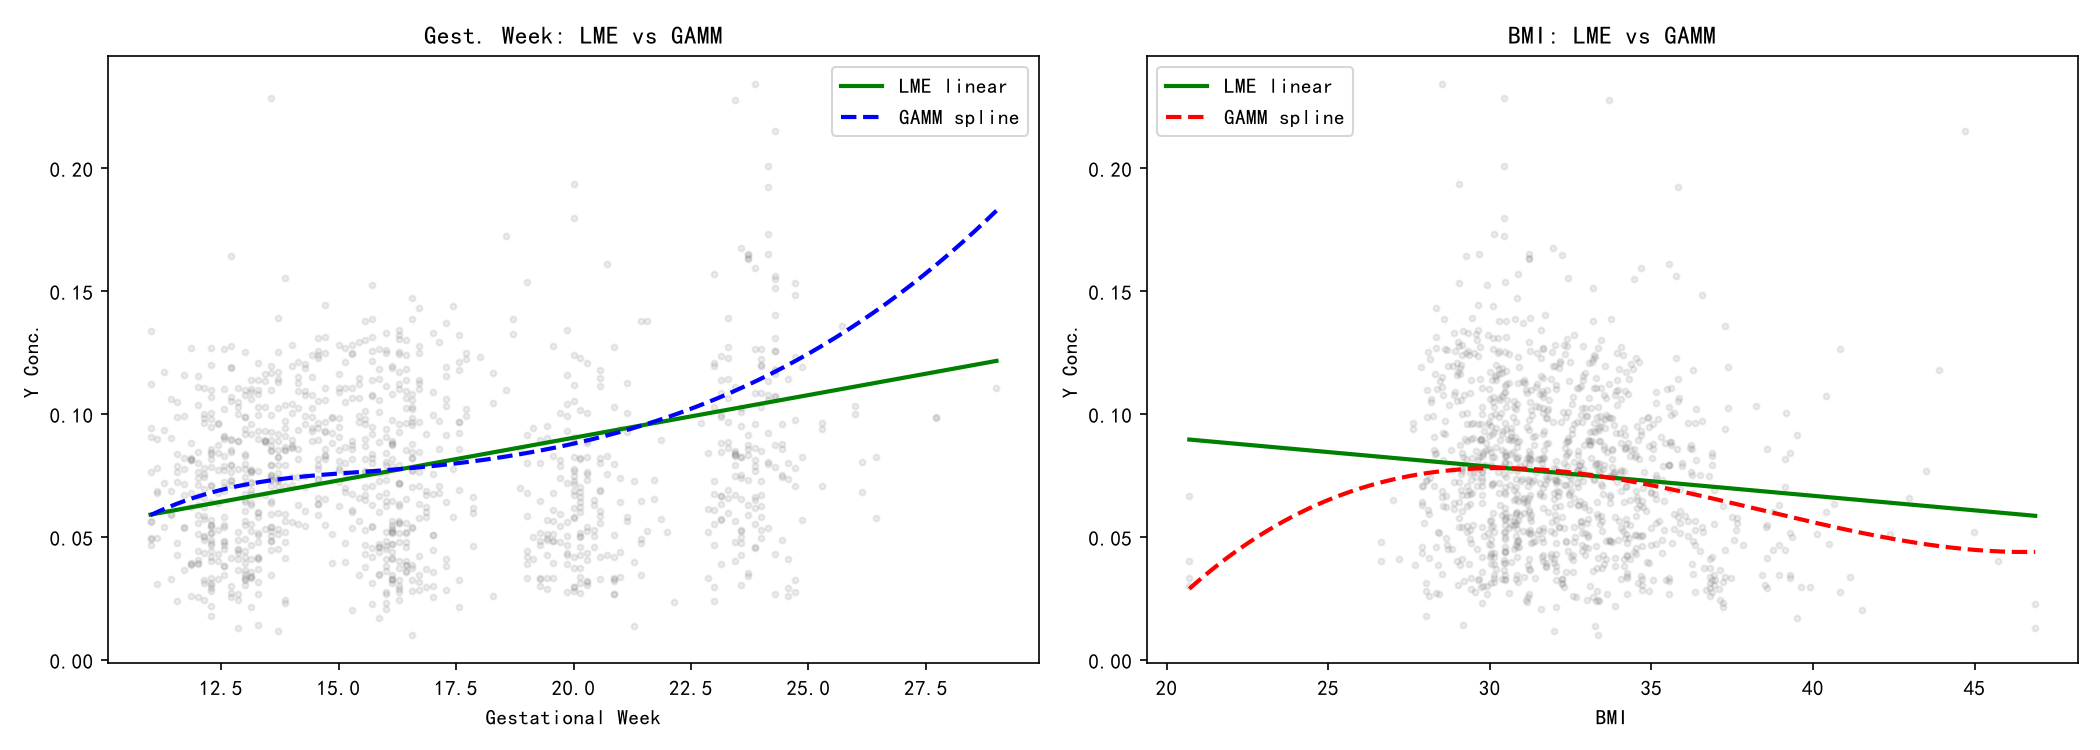
\includegraphics[width=0.85\textwidth]{Q1/experiments/round1/figures/M1_vs_M2_partial_effects.png}
  \caption{M1（GAMM）与M2（LME）偏效应对比}\label{fig:q1-partial}
\end{figure}

图~\ref{fig:q1-gest}给出GAMM模型中孕周偏效应的单独可视化及其95\%置信带。B样条基系数从早期的$0.0153$递增至$0.1238$，Y染色体浓度在孕早期增长平缓，中晚期后加速上升。这一非线性特征是GAMM相对于LME取得改进的核心来源。

\begin{figure}[H]
  \centering
  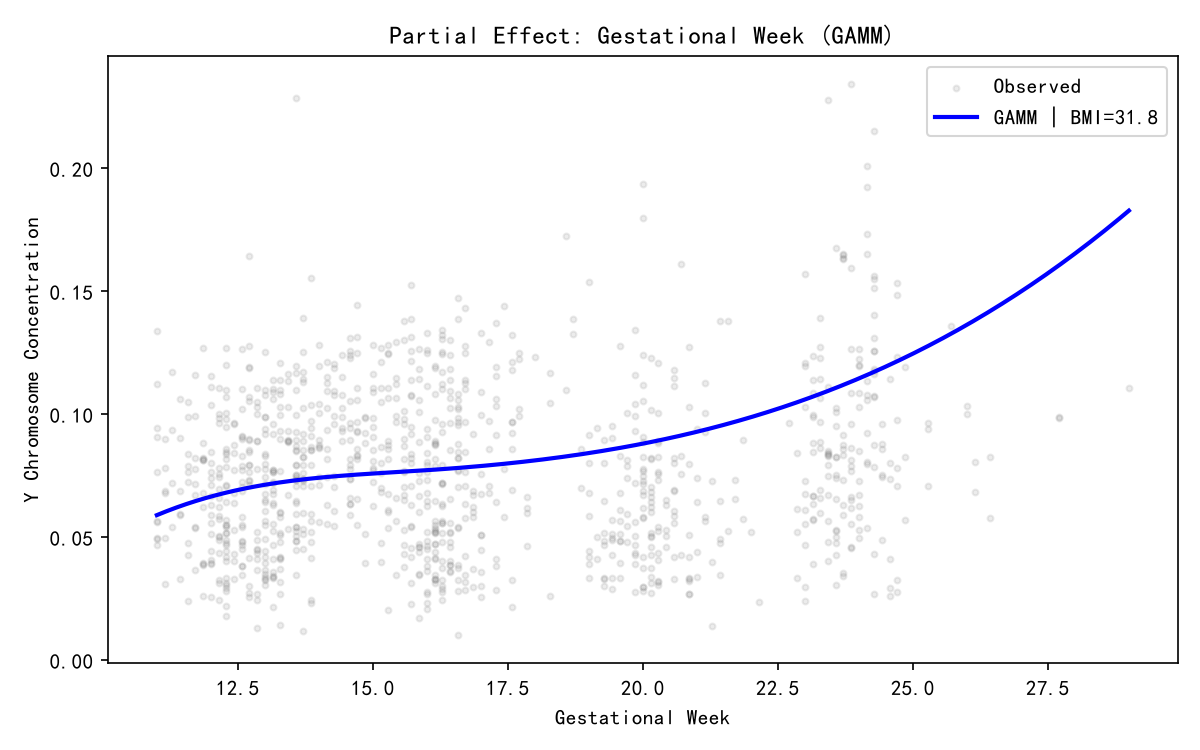
\includegraphics[width=0.75\textwidth]{Q1/experiments/round1/figures/M1_GAMM_partial_gest_week.png}
  \caption{GAMM模型孕周偏效应曲线}\label{fig:q1-gest}
\end{figure}

\subsection{结果分析}

GAMM的求解结果揭示了三条规律。

（1）孕周对Y染色体浓度具有强非线性正向效应。样条基系数序列$0.0153 \to 0.0173 \to 0.0434 \to 0.1238$表明浓度增速随孕周推进逐步加快，似然比检验（$\chi^2=76.76$，$p<10^{-15}$）证实这一非线性成分不可省略。

（2）BMI对Y染色体浓度存在负向调节作用。BMI样条基的首项系数$0.1023$后迅速回落至$0.0127$和$0.0150$，高BMI孕妇体内母体血浆体积增大，对胎儿游离DNA产生稀释效应，检测浓度偏低。

（3）个体异质性显著。ICC=0.60意味着超过半数的浓度变异归因于个体间差异，随机截距方差$\hat{\sigma}^2_{b0}=0.0019$远大于随机斜率方差$\hat{\sigma}^2_{b1}=0.000008$，不同孕妇的基线浓度水平差异是个体异质性的主要表现。

从NIPT临床实践角度看，孕周效应的非线性意味着对所有孕妇施行统一采样策略并非最优。孕早期浓度增速慢，过早采样可能因浓度不足而增加检测失败风险；孕中晚期浓度快速攀升，灵敏度相对充裕。BMI的稀释效应进一步加剧了这一问题，高BMI孕妇在相同孕周下浓度系统性偏低，需要推迟采样以补偿浓度劣势。这两项发现自然引出一个后续问题，即如何根据BMI水平制定分组化的最优检测时点，这正是问题二要回答的内容。


\section{问题二的建立与求解}

\subsection{数据驱动的BMI分组}

\subsubsection{选择依据}

不同BMI水平的孕妇，胎儿游离DNA浓度的增长速率存在差异，NIPT检测达标时间随BMI变化。若对全部孕妇采用统一检测时点，高BMI群体将面临较高的误检风险，需要按BMI水平分组并分别确定最优检测时点。传统做法依赖临床经验设定固定分界值，缺乏统计支撑。本文采用数据驱动策略，以组内达标时间方差最小化为目标，自动搜索最优分组断点。

\subsubsection{总述}

267名孕妇中，260名在观测期内Y染色体浓度首次达到检测阈值$c=0.04$（即4\%），据此定义经验达标时间$T^*$。对$T^*$关于BMI建立\textbf{Huber稳健回归}模型，在候选断点空间中穷举搜索，以BIC准则同时确定分组数目与断点位置。

\subsubsection{求解步骤}

\textbf{Step 1\quad 经验达标时间提取。}对每位孕妇的纵向浓度序列，取Y染色体浓度首次满足$\hat{y}(t) \geq 0.04$的孕周作为经验达标时间$T^*$。267名孕妇中有260名在观测窗口内达标，后续分析基于这260条记录。

\textbf{Step 2\quad 稳健回归建模。}以BMI为自变量，$T^*$为因变量，拟合二次稳健回归模型
\begin{equation}\label{eq:robust_reg}
  T^* = \beta_0 + \beta_1 \cdot \mathrm{BMI} + \beta_2 \cdot \mathrm{BMI}^2,
\end{equation}
采用Huber M-估计量以降低离群点的影响。图~\ref{fig:threshold_bmi}展示了$T^*$随BMI的变化趋势与拟合曲线。

\textbf{Step 3\quad 穷举断点搜索。}在BMI$\in[24,44]$范围内以步长1.0枚举所有候选断点组合，约束每组BMI宽度不少于3.0个单位、每组样本量不少于5人。对每种分组方案，计算组内$T^*$的加权方差，并以BIC准则评价模型复杂度与拟合优度的平衡。

\textbf{Step 4\quad 最优分组确定。}BIC最小方案对应两个断点BMI$=30$与BMI$=36$，将孕妇分为3组。临床经验5组方案（断点20/28/32/36/40）的BIC更高，额外分组并未带来组内方差的实质性下降。

\begin{figure}[H]
  \centering
  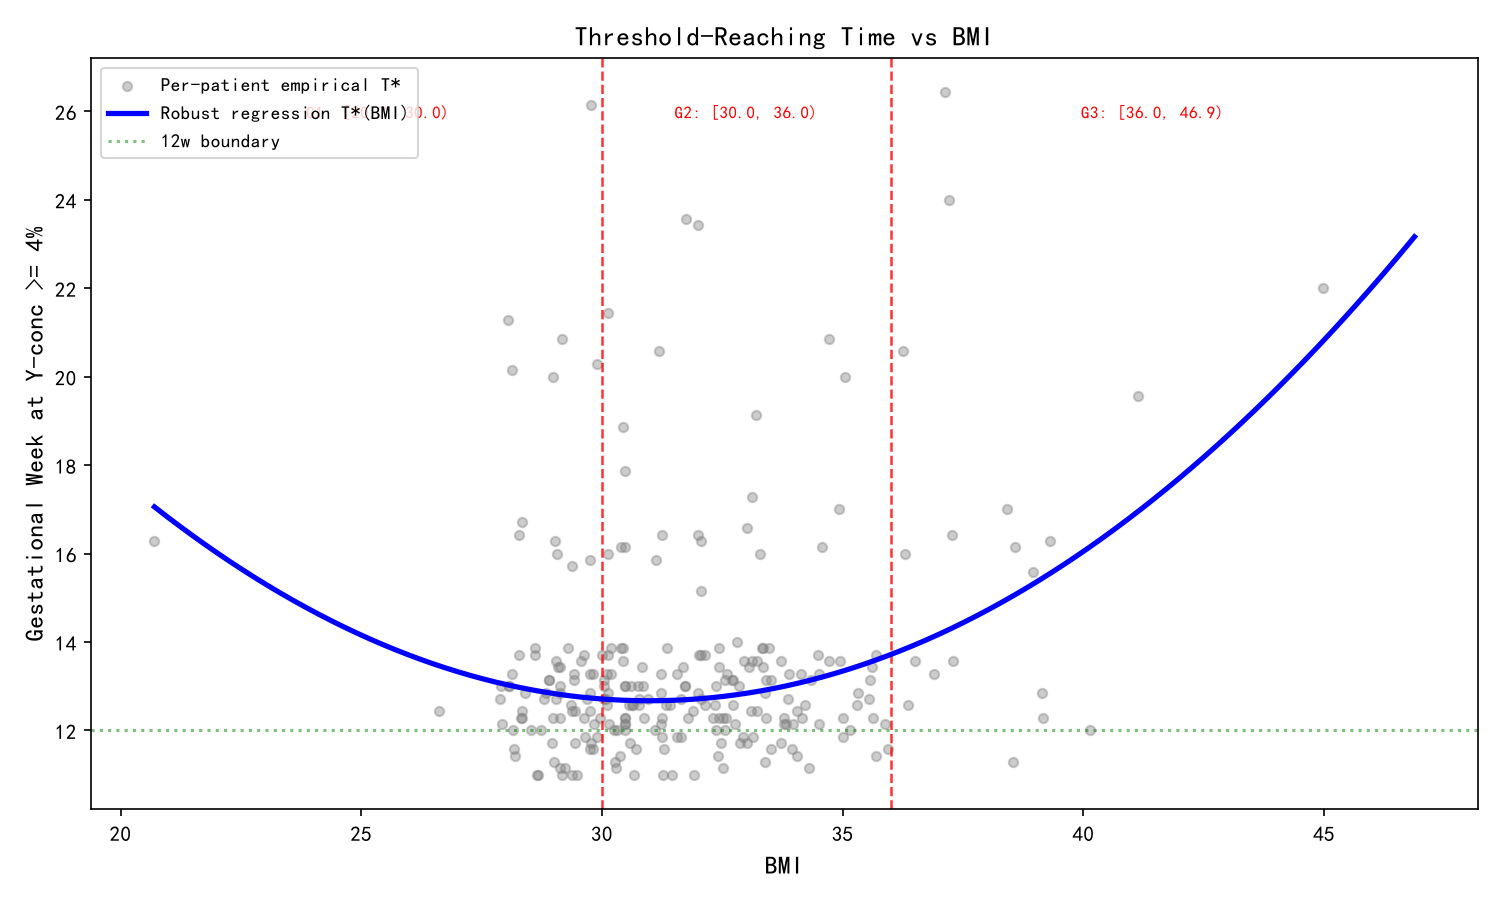
\includegraphics[width=0.85\textwidth]{Q2/experiments/round1/figures/M1_threshold_time_vs_bmi.png}
  \caption{经验达标时间$T^*$与BMI的关系及稳健回归拟合曲线，竖线标注最优断点}\label{fig:threshold_bmi}
\end{figure}

\subsection{风险函数的建立}

\subsubsection{选择依据}

NIPT检测时点的选择涉及两类竞争风险。检测过早，胎儿游离DNA浓度尚未充分积累，准确性不足；检测过晚，则延误临床干预窗口。需要构造统一的风险函数，将两类风险量化并加权求和，为最优时点求解提供目标函数。

\subsubsection{总述}

定义总风险函数为延迟风险与不准确风险的加权和，其中不准确风险基于问题一的GAMM预测值与残差标准差，通过正态累积分布函数刻画浓度低于阈值的概率。

\subsubsection{模型构建}

总风险函数定义为
\begin{equation}\label{eq:total_risk}
  R(t,\mathrm{BMI}) = w_d \cdot R_{\text{delay}}(t) + w_a \cdot R_{\text{inacc}}(t,\mathrm{BMI}),
\end{equation}
其中$w_d=0.4$，$w_a=0.6$，反映临床实践中检测准确性的优先级高于时效性。

延迟风险采用Sigmoid函数建模
\begin{equation}\label{eq:delay_risk}
  R_{\text{delay}}(t) = \frac{1}{1+e^{-0.5(t-18)}},
\end{equation}
该函数在孕18周附近快速上升，刻画超过常规检测窗口后临床干预机会急剧减少的特征。

不准确风险基于GAMM预测浓度$\hat{y}(t,\mathrm{BMI})$与残差标准差$\sigma_\varepsilon=0.0101$，通过标准正态累积分布函数$\Phi$计算浓度低于检测阈值$c=0.04$的概率
\begin{equation}\label{eq:inacc_risk}
  R_{\text{inacc}}(t,\mathrm{BMI}) = \Phi\!\left(\frac{c - \hat{y}(t,\mathrm{BMI})}{\sigma_\varepsilon}\right).
\end{equation}

当预测浓度远高于阈值时，$R_{\text{inacc}}$趋近于0；当预测浓度接近或低于阈值时，$R_{\text{inacc}}$迅速增大。图~\ref{fig:risk_analysis}展示了两类风险分量及总风险随孕周的变化。

\begin{figure}[H]
  \centering
  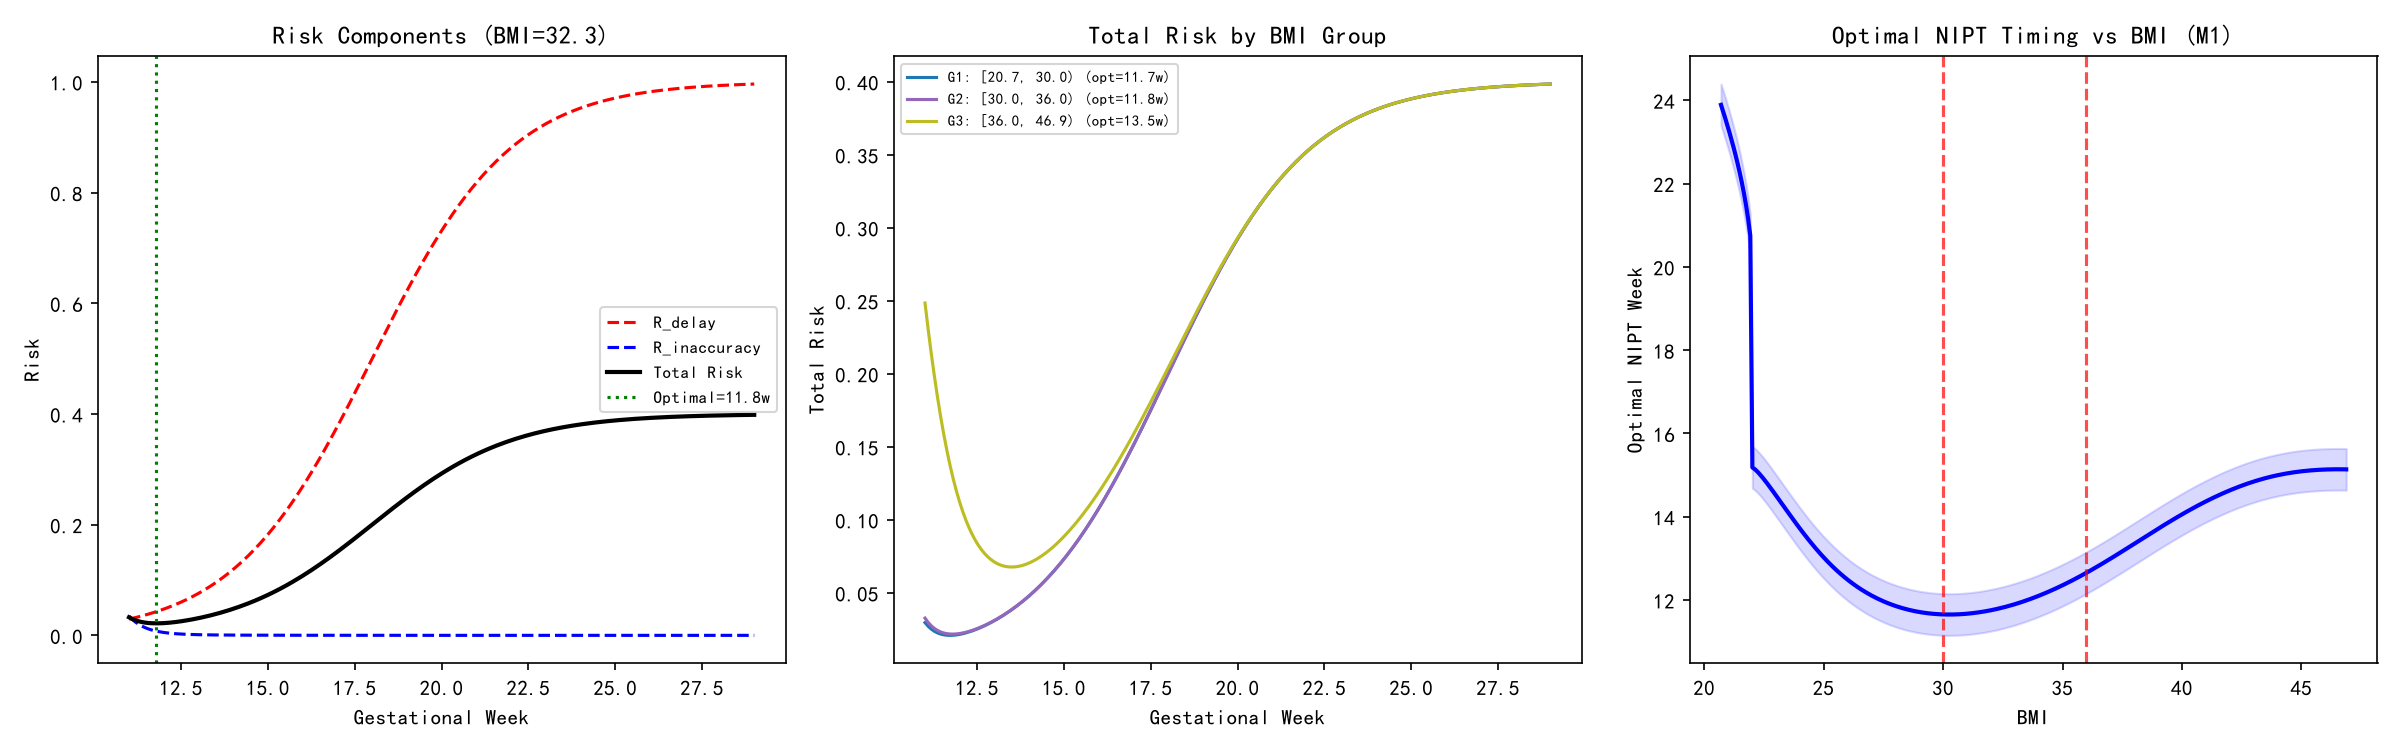
\includegraphics[width=0.85\textwidth]{Q2/experiments/round1/figures/M1_risk_function_analysis.png}
  \caption{各BMI组的风险函数分析，延迟风险、不准确风险及总风险随孕周的变化}\label{fig:risk_analysis}
\end{figure}

\subsection{最优检测时点求解}

\subsubsection{选择依据}

风险函数$R(t,\mathrm{BMI})$在孕周$t$上呈先降后升的"U形"结构，早期以不准确风险为主导，晚期以延迟风险为主导。两类风险的交汇区域对应总风险最低的检测窗口，该最低点即为各组最优检测时点。

\subsubsection{求解方法}

对第$g$组，取该组BMI均值$\overline{\mathrm{BMI}}_g$代入风险函数，在孕周区间$[10,25]$上求解单变量有界优化问题
\begin{equation}\label{eq:opt_time}
  T_g^* = \arg\min_{t\in[10,25]} R(t,\,\overline{\mathrm{BMI}}_g),
\end{equation}
使用Brent方法（scipy.optimize.minimize\_scalar）进行精确求解。

\subsubsection{求解结果}

三组的最优检测时点及对应风险值列于表~\ref{tab:opt_results}。

\begin{table}[H]
  \centering
  \caption{各BMI组最优检测时点与风险值}\label{tab:opt_results}
  \begin{tabular}{cccccc}
    \toprule
    组别 & BMI范围 & 样本量 & BMI均值 & 最优孕周 & 最小风险 \\
    \midrule
    G1 & $[20.7,\,30.0)$ & 76  & 28.9 & 11.72 & 0.0208 \\
    G2 & $[30.0,\,36.0)$ & 171 & 32.3 & 11.80 & 0.0218 \\
    G3 & $[36.0,\,46.9)$ & 20  & 38.4 & 13.49 & 0.0675 \\
    \bottomrule
  \end{tabular}
\end{table}

G1与G2组的最优时点十分接近（约11.7$\sim$11.8周），最小风险均低于0.025，中低BMI孕妇在孕12周前即可获得高置信度的检测结果。G3组（BMI$\geq$36）的最优时点推迟至13.49周，最小风险升高至0.0675，约为前两组的3倍。高BMI孕妇的母体游离DNA对胎儿DNA的稀释效应更强，浓度达标时间整体后移。

经验达标时间的中位数（G1为12.79周、G2为12.71周、G3为16.00周）均晚于模型给出的最优时点，基于风险函数的最优解能够在保证准确性的前提下提前检测窗口。

\subsection{检测误差敏感性分析}

\subsubsection{分析目的}

实际检测中，仪器精度与样本处理过程均可能引入系统偏差或随机噪声。需要评估检测阈值偏移或残差方差增大时，各组最优时点与最小风险的稳定性。

\subsubsection{扰动设计}

设置两类扰动实验。

（1）阈值偏移。将检测阈值$c$分别上调0.5\%、1\%、2\%（即$c=0.045$、$0.05$、$0.06$），模拟系统性测量偏差。

（2）噪声膨胀。将残差标准差$\sigma_\varepsilon$分别放大至1.5倍、2倍、3倍（即$\sigma_\varepsilon=0.0152$、$0.0202$、$0.0303$），模拟随机误差增大的场景。

\subsubsection{敏感性结果}

图~\ref{fig:sensitivity}展示了各组在不同扰动水平下的风险响应。G1和G2组在所有扰动条件下，最优时点偏移不超过0.5周，最小风险增幅有限，鲁棒性较好。G3组对两类扰动均敏感，噪声放大至3倍时最小风险超过0.15，最优时点进一步推迟。这与高BMI组信噪比偏低的物理机制一致，浓度预测的不确定性在高BMI区间被放大。

\begin{figure}[H]
  \centering
  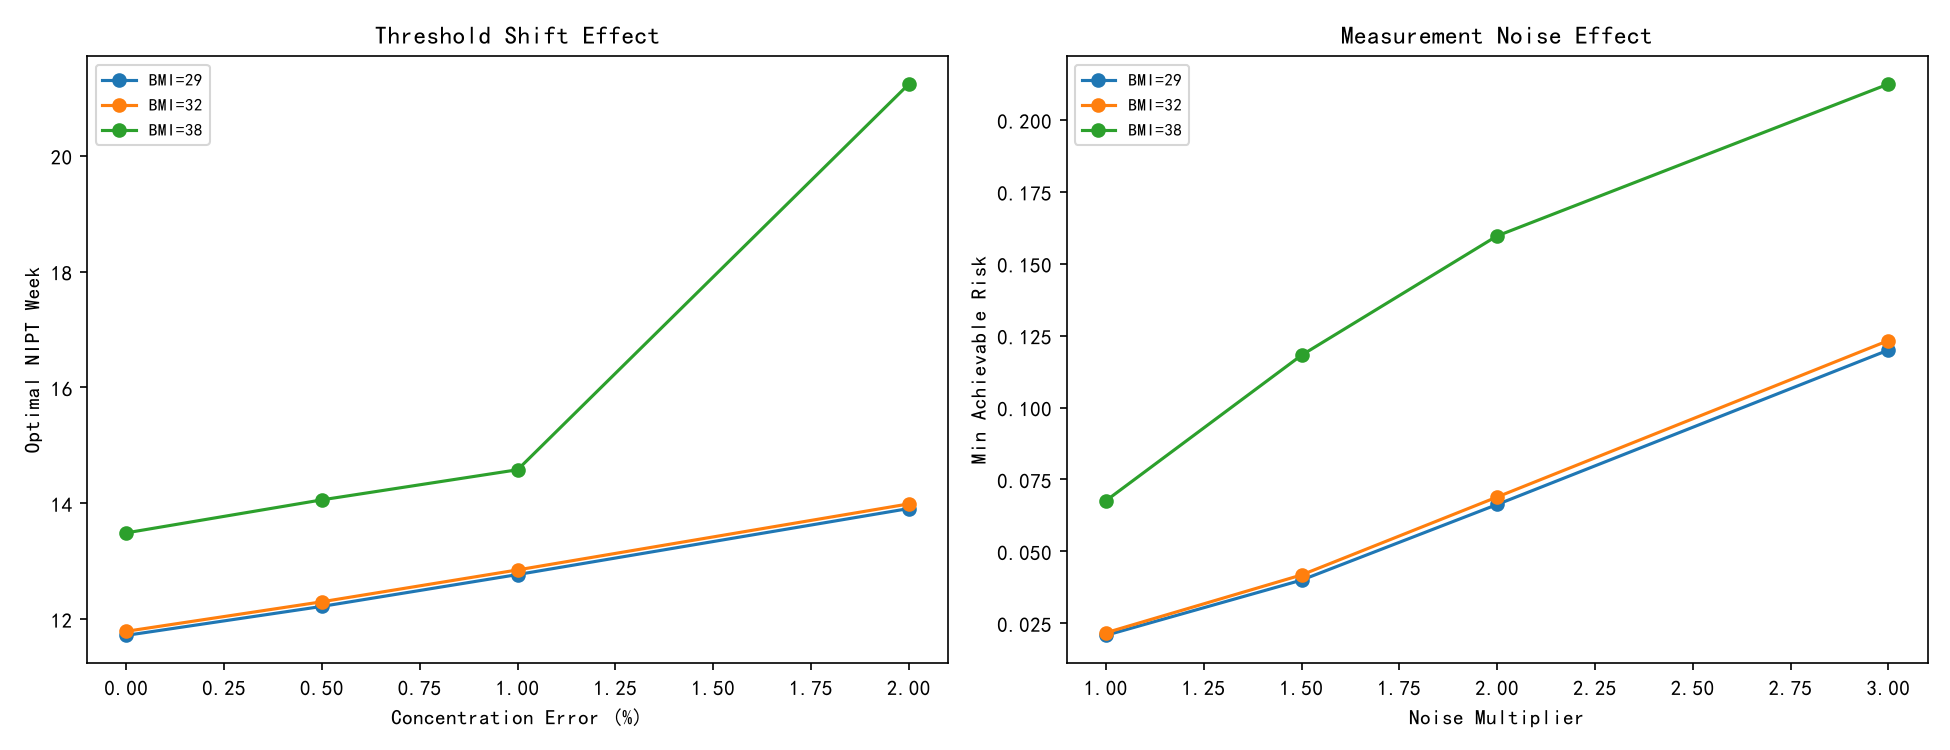
\includegraphics[width=0.85\textwidth]{Q2/experiments/round1/figures/M1_error_sensitivity.png}
  \caption{检测误差敏感性分析，阈值偏移与噪声膨胀对各组风险的影响}\label{fig:sensitivity}
\end{figure}

作为对照，临床经验5组方案（M2，断点为BMI$=$20/28/32/36/40）给出的最优检测时点分布在11.65$\sim$14.65周之间，趋势与数据驱动方案一致，但额外的分组未能带来风险的明显降低，验证了BIC准则选择3组方案的合理性。

\subsection{实际意义}

上述结果为临床NIPT检测方案的制定提供了量化参考。BMI低于30的孕妇（占样本的28.5\%）和BMI在30$\sim$36之间的孕妇（占64.0\%）可在孕11$\sim$12周安全接受检测，风险水平低于0.025。BMI超过36的孕妇（占7.5\%）应将检测时点推迟至约13.5周，临床解读时需考虑该群体面临的较高检测不确定性。对于高BMI孕妇，在条件允许时可考虑重复采样或联合其他产前筛查手段，以弥补单次NIPT信噪比不足的问题。


\section{问题三的建立与求解}

问题一和问题二的模型仅纳入孕周与BMI两个因素。问题三进一步考察年龄和体重对Y染色体浓度预测的增量贡献，并在多因素框架下重新优化分组检测时点。由于体重、身高与BMI之间存在严重的多重共线性，直接纳入将导致参数估计不稳定，需要先进行变量解耦。

\subsection{多重共线性诊断与残差分解}

\subsubsection{共线性诊断}

将体重、身高、BMI和年龄同时纳入线性模型，计算各变量的方差膨胀因子（VIF）。VIF衡量自变量间线性相关对回归系数方差的放大倍数，定义为
\begin{equation}\label{eq:vif}
  \mathrm{VIF}_k = \frac{1}{1 - R_k^2}
\end{equation}

其中$R_k^2$为第$k$个自变量对其余自变量回归的决定系数。通常以$\mathrm{VIF} > 10$作为严重共线性的判据。原始变量的VIF结果如表~\ref{tab:vif_before}所示。

\begin{table}[H]
  \caption{残差分解前各变量的VIF}
  \label{tab:vif_before}
  \centering
  \begin{tabular}{lcccc}
    \hline
    变量 & BMI & 身高 & 体重 & 年龄 \\
    \hline
    VIF & 218.6 & 106.9 & 351.3 & 1.01 \\
    \hline
  \end{tabular}
\end{table}

BMI、身高和体重三者的VIF均远超10，直接建模将使系数估计高度不稳定。

\subsubsection{残差分解策略}

为保留体重中独立于BMI和身高的信息，本文采用残差分解法。将体重对BMI和身高进行辅助回归
\begin{equation}\label{eq:resid_decomp}
  \text{weight}_i = \gamma_0 + \gamma_1 \cdot \mathrm{BMI}_i + \gamma_2 \cdot \text{height}_i + e_i
\end{equation}

残差$e_i$即为体重中无法被BMI和身高线性解释的部分，记为$\text{weight\_resid}_i$。以BMI、年龄和$\text{weight\_resid}$替换原始变量后，重新计算VIF，结果如表~\ref{tab:vif_after}所示。

\begin{table}[H]
  \caption{残差分解后各变量的VIF}
  \label{tab:vif_after}
  \centering
  \begin{tabular}{lccc}
    \hline
    变量 & BMI & 年龄 & weight\_resid \\
    \hline
    VIF & 1.00 & 1.01 & 1.01 \\
    \hline
  \end{tabular}
\end{table}

分解后所有VIF均接近1，共线性问题完全消除。图~\ref{fig:vif_comparison}直观展示了分解前后VIF的对比。

\begin{figure}[H]
  \centering
  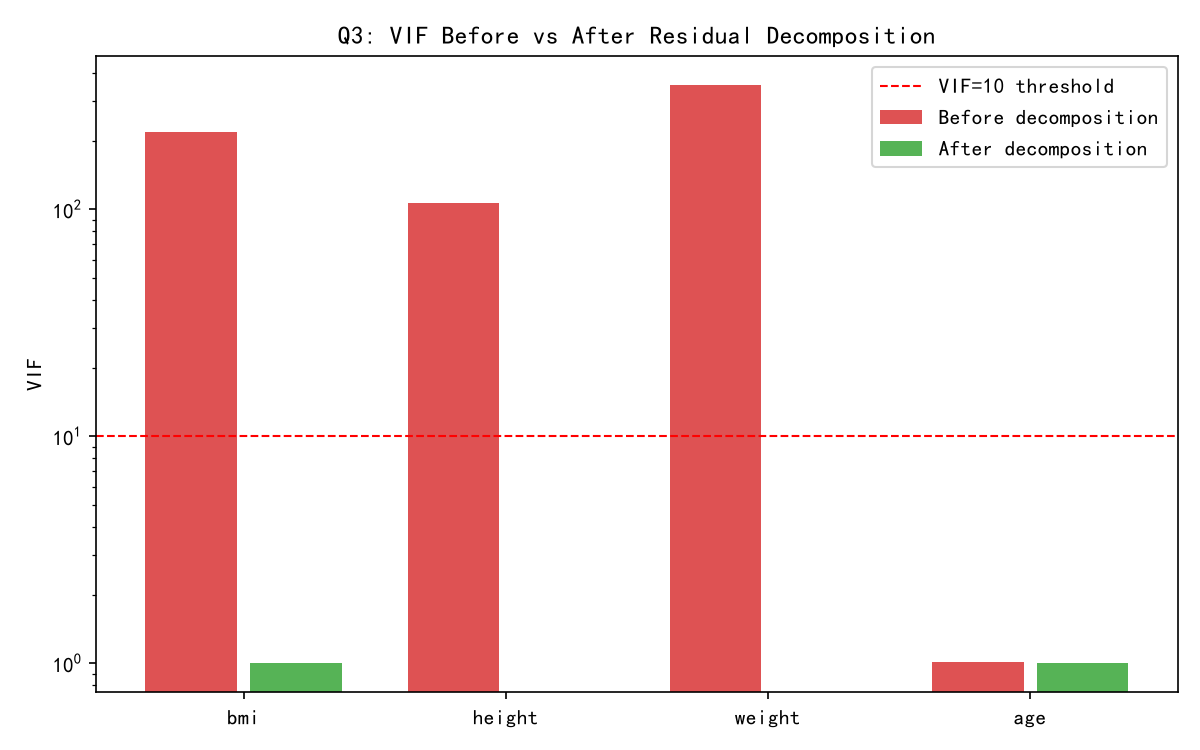
\includegraphics[width=0.85\textwidth]{Q3/experiments/round1/figures/q3_vif_comparison.png}
  \caption{残差分解前后各变量VIF对比}
  \label{fig:vif_comparison}
\end{figure}

\subsection{多因素GAMM模型}

\subsubsection{模型建立}

在问题一GAMM的基础上，将年龄和体重残差作为线性固定效应纳入，建立\textbf{多因素广义加性混合模型（Multi-factor GAMM，记为M1）}
\begin{equation}\label{eq:gamm_q3}
  y_{ij} = \beta_0 + s_1(t_{ij}) + s_2(\mathrm{BMI}_i) + \beta_3 \cdot \text{age}_i + \beta_4 \cdot \text{weight\_resid}_i + b_{0i} + b_{1i}\,t_{ij} + \varepsilon_{ij}
\end{equation}

其中各成分含义如下。

\begin{itemize}
  \item $s_1(\cdot)$、$s_2(\cdot)$分别为孕周和BMI的非线性平滑函数，沿用问题一的B样条基设定；
  \item $\beta_3$为年龄的线性效应系数；
  \item $\beta_4$为体重残差的线性效应系数；
  \item $b_{0i}$、$b_{1i}$分别为随机截距和随机斜率，刻画个体异质性；
  \item $\varepsilon_{ij} \sim N(0,\,\sigma^2_\varepsilon)$为观测误差。
\end{itemize}

作为对照，建立\textbf{基准模型（M2）}，仅保留年龄和BMI与年龄的交互项
\begin{equation}\label{eq:gamm_q3_m2}
  y_{ij} = \beta_0 + s_1(t_{ij}) + s_2(\mathrm{BMI}_i) + \beta_3 \cdot \text{age}_i + \beta_5 \cdot (\mathrm{BMI}_i \times \text{age}_i) + b_{0i} + b_{1i}\,t_{ij} + \varepsilon_{ij}
\end{equation}

\subsubsection{模型求解与比较}

模型估计按以下步骤执行。

\textbf{Step 1}（残差分解）\quad 对267名孕妇的体重执行式~\eqref{eq:resid_decomp}的辅助回归，提取残差$\text{weight\_resid}$，与BMI、年龄共同构成正交化自变量集。

\textbf{Step 2}（参数估计）\quad 采用REML估计M1和M2的方差成分与固定效应参数，平滑函数的惩罚参数通过广义交叉验证（GCV）自动选取。

\textbf{Step 3}（信息准则比较）\quad 分别计算两个模型的AIC，评估新增变量的预测增益。

\textbf{Step 4}（系数显著性检验）\quad 对M1中年龄和体重残差的线性系数进行$t$检验，判断其统计显著性。

模型比较结果如表~\ref{tab:q3_model_compare}所示。

\begin{table}[H]
  \caption{多因素GAMM模型比较}
  \label{tab:q3_model_compare}
  \centering
  \begin{tabular}{lcc}
    \hline
    模型 & 描述 & AIC \\
    \hline
    M1 & GAMM + age + weight\_resid & $-5214.43$ \\
    M2 & GAMM + age + BMI$\times$age & $-5208.70$ \\
    \hline
  \end{tabular}
\end{table}

M1的AIC略优于M2，但两者差距仅为5.73，改善幅度有限。M1中新增线性项的系数估计如表~\ref{tab:q3_coef}所示。

\begin{table}[H]
  \caption{M1模型中年龄与体重残差的系数估计}
  \label{tab:q3_coef}
  \centering
  \begin{tabular}{lccc}
    \hline
    变量 & 系数 & 标准误 & $p$值 \\
    \hline
    age & $-0.000491$ & $0.000482$ & 0.309 \\
    weight\_resid & $-0.001020$ & $0.002514$ & 0.685 \\
    \hline
  \end{tabular}
\end{table}

两个变量的$p$值均远大于0.05，未达到统计显著性。BMI的非线性样条效应在M1中仍为最主要的预测成分，其有效自由度和$F$统计量与问题一模型基本一致。

这一结果表明，在已纳入BMI非线性效应的条件下，年龄和体重（扣除BMI和身高的线性贡献后）对Y染色体浓度不具有显著的额外预测能力。BMI已充分捕获了体脂水平对胎儿游离DNA稀释效应的影响。

\subsection{达标比例与风险优化}

\subsubsection{风险函数构建}

问题二的最优时点仅基于群体预测均值确定，未考虑个体间预测分布的离散程度。为更全面地权衡检测时机，本文定义达标比例（compliance rate）为BMI分组$g$在孕周$t$时，预测Y染色体浓度不低于检测阈值$c=0.04$的个体占比
\begin{equation}\label{eq:compliance}
  P(y \geq 0.04 \mid t,\, g) = \frac{1}{N_g} \sum_{i \in g} \mathbf{1}\!\left[\hat{y}_i(t) \geq 0.04\right]
\end{equation}

其中$\hat{y}_i(t)$由GAMM预测均值叠加随机效应采样和残差噪声生成，通过Monte Carlo模拟获得。

同时定义延迟检测风险$R_{\text{late}}(t)$为分段线性函数
\begin{equation}\label{eq:late_risk}
  R_{\text{late}}(t) = \begin{cases}
    0, & t \leq 12 \\[4pt]
    \displaystyle\frac{0.5\,(t-12)}{20-12}, & 12 < t \leq 20 \\[6pt]
    \displaystyle 0.5 + \frac{0.5\,(t-20)}{25-20}, & 20 < t \leq 25
  \end{cases}
\end{equation}

该函数反映临床实践中检测时点越晚，后续干预窗口越窄所带来的风险递增。综合两项指标，构建加权风险函数
\begin{equation}\label{eq:risk_func}
  R(t,\,g) = 0.3 \cdot R_{\text{late}}(t) + 0.7 \cdot \bigl(1 - P(y \geq 0.04 \mid t,\,g)\bigr)
\end{equation}

权重分配体现了达标比例（即检测灵敏度）对NIPT决策的优先地位，同时兼顾延迟风险的临床约束。

\subsubsection{分组优化结果}

沿用问题二的临床知情BMI分组策略（最小组容量$n_{\min}=10$），将267名孕妇划分为4组，对每组在$t \in [11, 25]$周的网格上逐点计算$R(t,g)$，取最小值对应的孕周为最优检测时点。结果如表~\ref{tab:q3_optimal}所示。

\begin{table}[H]
  \caption{各BMI组的最优检测时点与达标比例}
  \label{tab:q3_optimal}
  \centering
  \begin{tabular}{ccccc}
    \hline
    BMI分组 & 样本量 & 最优孕周 & 达标比例 & 最小风险值 \\
    \hline
    $[20, 32)$ & 152 & 12.8 & 75.3\% & 0.187 \\
    $[32, 36)$ & 95  & 13.3 & 74.8\% & 0.200 \\
    $[36, 40)$ & 16  & 13.3 & 67.0\% & 0.256 \\
    $[40, +\infty)$ & 4 & 24.8 & 95.0\% & 0.329 \\
    \hline
  \end{tabular}
\end{table}

前三组的最优时点集中在12.8至13.3周，与问题二的结论基本吻合。BMI$\geq$40组的最优时点被推迟至24.8周，原因在于该组胎儿游离DNA浓度增长极为缓慢，在12至20周区间内达标比例始终偏低，风险函数直到接近观测窗口上限才取得最小值。图~\ref{fig:compliance_curves}展示了各组达标比例随孕周的变化趋势。

\begin{figure}[H]
  \centering
  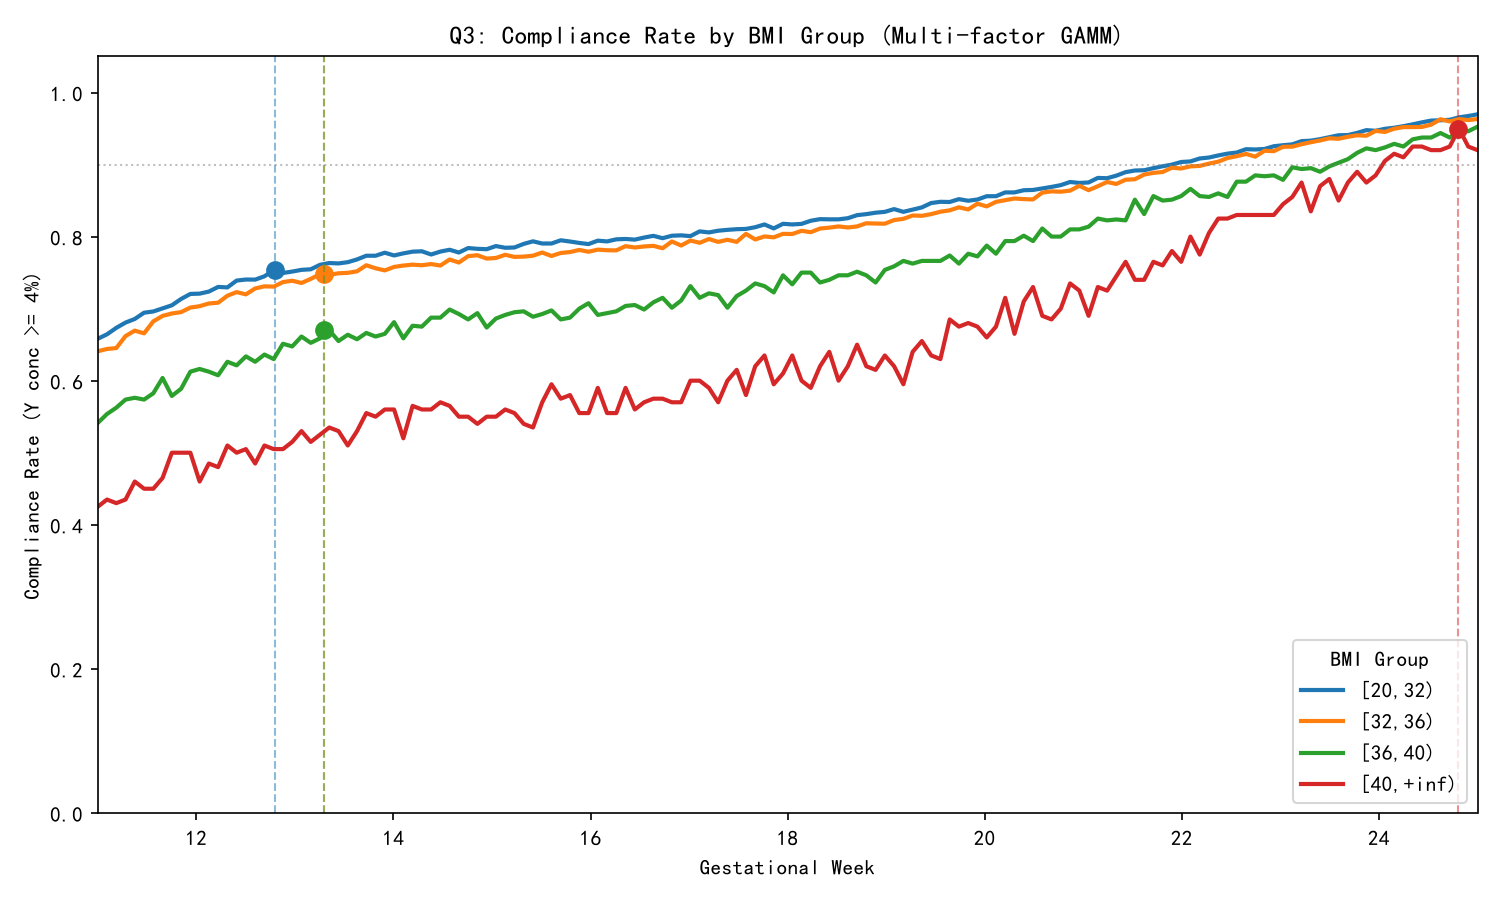
\includegraphics[width=0.85\textwidth]{Q3/experiments/round1/figures/q3_compliance_curves.png}
  \caption{各BMI组达标比例随孕周变化曲线}
  \label{fig:compliance_curves}
\end{figure}

\subsection{Monte Carlo误差传播分析}

\subsubsection{分析动机与方法}

上述最优时点的确定依赖于GAMM的点估计和固定的残差方差$\sigma^2_\varepsilon$。测量噪声的实际水平存在不确定性，可能影响达标比例的计算进而改变最优时点的位置。为量化这一不确定性，本文采用Monte Carlo误差传播方法，在不同噪声水平下重复优化过程，获得最优时点的经验分布。

具体步骤如下。

\textbf{Step 1}（噪声扰动）\quad 设模型估计的残差标准差为$\hat{\sigma}_\varepsilon$。在每次Monte Carlo迭代中，从均匀分布$U(0.5,\,1.5)$中抽取缩放因子$\lambda$，将残差标准差设为$\lambda \hat{\sigma}_\varepsilon$，模拟测量精度在$0.5$倍至$1.5$倍范围内波动的情形。

\textbf{Step 2}（重新优化）\quad 在扰动后的噪声水平下，重新执行达标比例的Monte Carlo模拟，并对每个BMI组重新搜索使式~\eqref{eq:risk_func}最小的孕周。

\textbf{Step 3}（分布统计）\quad 重复上述过程500次，收集每个BMI组最优时点的经验分布，计算均值、标准差和95\%置信区间。

\subsubsection{误差传播结果}

500次Monte Carlo迭代的结果如表~\ref{tab:q3_mc}所示。

\begin{table}[H]
  \caption{Monte Carlo误差传播下各BMI组最优时点的分布统计}
  \label{tab:q3_mc}
  \centering
  \begin{tabular}{ccccc}
    \hline
    BMI分组 & 均值（周） & 标准差（周） & 95\%置信区间 \\
    \hline
    $[20, 32)$      & 13.02 & 0.64 & $[11.94,\; 14.34]$ \\
    $[32, 36)$      & 13.17 & 0.81 & $[11.94,\; 15.00]$ \\
    $[36, 40)$      & 14.47 & 3.04 & $[11.38,\; 23.64]$ \\
    $[40, +\infty)$ & 16.15 & 4.75 & $[11.00,\; 24.58]$ \\
    \hline
  \end{tabular}
\end{table}

图~\ref{fig:mc_distributions}展示了各组最优时点在500次迭代中的经验分布。

\begin{figure}[H]
  \centering
  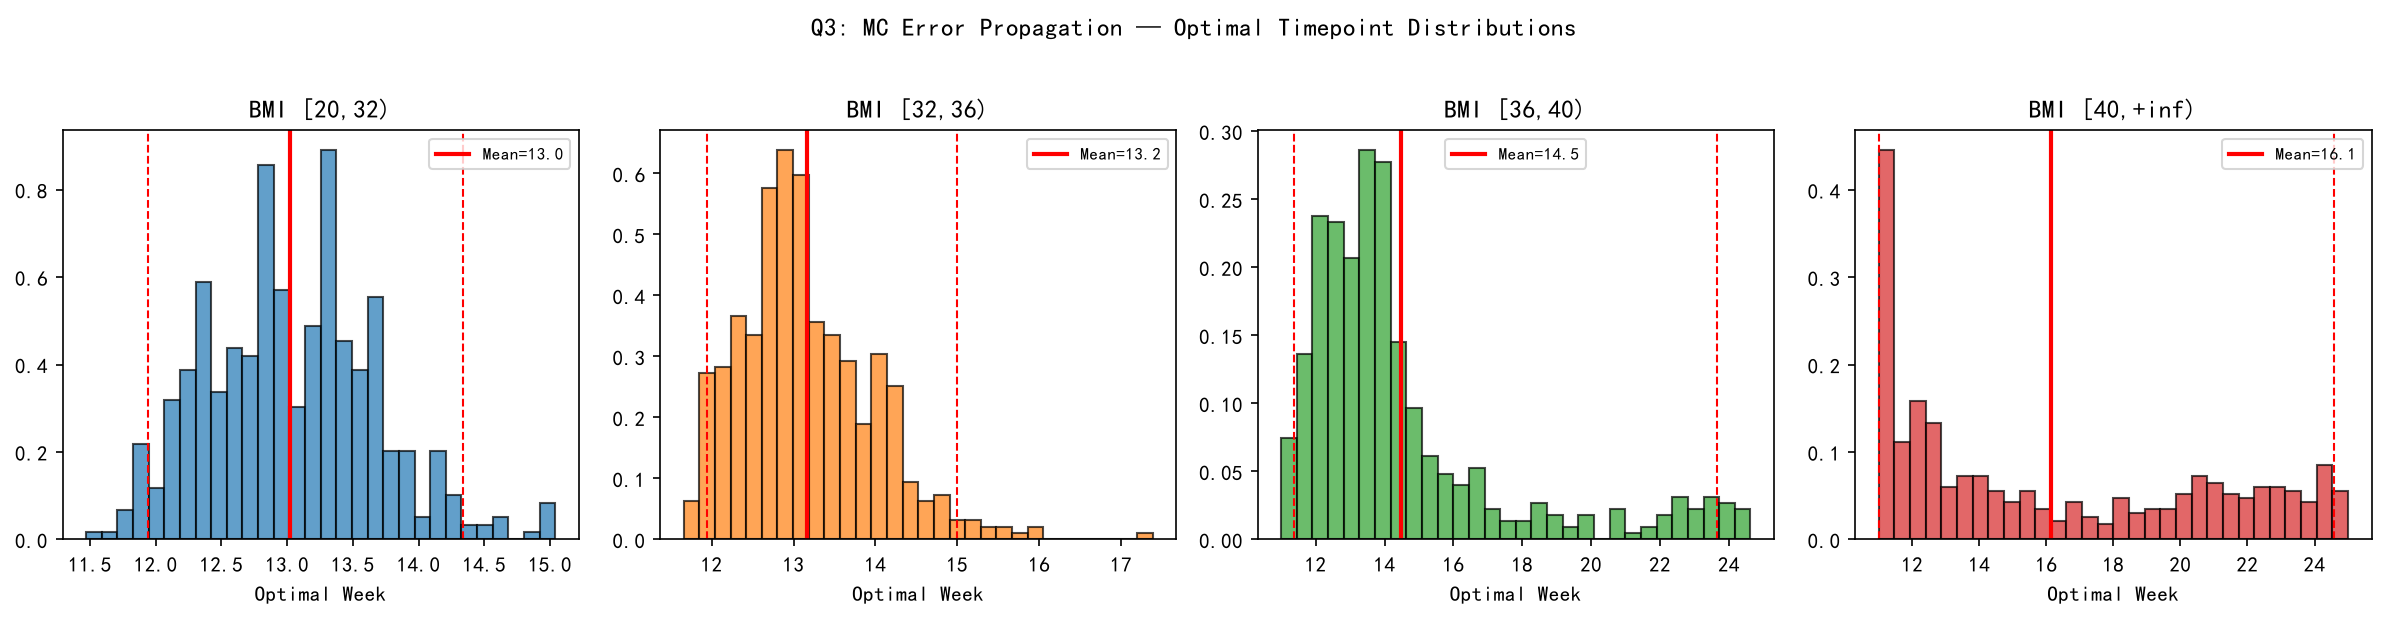
\includegraphics[width=0.85\textwidth]{Q3/experiments/round1/figures/q3_mc_timepoint_distributions.png}
  \caption{Monte Carlo模拟下各BMI组最优检测时点的经验分布}
  \label{fig:mc_distributions}
\end{figure}

BMI在$[20, 32)$和$[32, 36)$两组的最优时点分布集中，标准差分别为0.64周和0.81周，95\%置信区间宽度不超过3.1周，表明这两组的时点推荐具有良好的稳健性。BMI在$[36, 40)$组的标准差增至3.04周，置信区间跨度达12.3周，推荐精度明显下降。BMI$\geq$40组的置信区间从11.0周延伸至24.6周，跨度达13.6周，最优时点在测量噪声扰动下几乎不可确定。该组仅包含4名孕妇，样本量的严重不足是导致估计不稳定的根本原因。

\subsection{实际意义}

问题三的分析为NIPT临床实践提供了三项定量依据。

第一，年龄和体重（在控制BMI之后）对Y染色体浓度不具有显著的额外预测能力。临床采集BMI即可充分刻画母体因素对胎儿游离DNA稀释效应的影响，无需额外采集或建模其他人体测量指标，可简化检测前的信息采集流程。

第二，BMI低于36的孕妇群体（占样本的92.5\%），基于达标比例与延迟风险联合优化的最优检测时点稳定在12.8至13.3周，Monte Carlo分析确认该推荐在测量噪声波动下具有充分的可靠性。

第三，BMI$\geq$36尤其是BMI$\geq$40的高BMI群体，最优时点的不确定性极大，当前样本量不足以支撑可靠的时点推荐。对这部分人群，建议在扩大样本的前提下重新评估，同时在临床决策中对单一模型输出保持审慎态度。


\section{问题四的建立与求解}

本题针对女性胎儿样本，由于缺少Y染色体标记，无法沿用前述基于Y染色体浓度的分析路径。需要利用NIPT检测的多维汇总统计量，建立染色体非整倍体异常（13-三体、18-三体、21-三体及性染色体异常）的检测模型。数据集包含604例女性胎儿样本，其中正常537例、异常67例，异常率约为11.1\%。

\subsection{问题转化与特征选择}

女性胎儿不携带Y染色体，前三个问题的Y染色体浓度建模思路不再适用。问题四的核心任务转化为，在多维NIPT汇总指标空间中将异常样本与正常样本区分开来。

候选特征涵盖各目标染色体的Z值、BMI、X染色体浓度、GC含量、读段计数及比对率等。经初步相关性分析与临床意义筛选，确定以下6个核心特征构成输入空间。

\begin{itemize}
  \item 13号染色体Z值（$Z_{13}$）、18号染色体Z值（$Z_{18}$）、21号染色体Z值（$Z_{21}$）
  \item X染色体Z值（$Z_X$）
  \item 孕妇BMI
  \item X染色体浓度
\end{itemize}

该特征集覆盖了三种常见常染色体三体及性染色体异常的直接度量指标，同时纳入BMI和X染色体浓度作为辅助变量，以捕捉母体特征对检测结果的潜在调节作用。

\subsection{多元马氏距离异常检测模型}

\subsubsection{模型建立}

本文建立\textbf{多元马氏距离异常检测模型（记为M1）}作为主方法。其基本思路为，以正常样本的多维分布为参照，计算每个待检样本偏离正常群体中心的马氏距离，距离越大则异常可能性越高。

设正常样本集为$\{\mathbf{x}_k\}_{k=1}^{n_0}$，其中$\mathbf{x}_k \in \mathbb{R}^6$为6维特征向量。首先估计正常群体的均值向量$\boldsymbol{\mu}$和协方差矩阵$\boldsymbol{\Sigma}$
\begin{equation}
  \boldsymbol{\mu} = \frac{1}{n_0}\sum_{k=1}^{n_0}\mathbf{x}_k, \qquad
  \boldsymbol{\Sigma} = \frac{1}{n_0-1}\sum_{k=1}^{n_0}(\mathbf{x}_k - \boldsymbol{\mu})(\mathbf{x}_k - \boldsymbol{\mu})^T
\end{equation}

对任意待检样本$\mathbf{x}$，其马氏距离定义为
\begin{equation}\label{eq:mahal}
  d_M(\mathbf{x}) = \sqrt{(\mathbf{x} - \boldsymbol{\mu})^T \boldsymbol{\Sigma}^{-1} (\mathbf{x} - \boldsymbol{\mu})}
\end{equation}

分类规则为，若$d_M(\mathbf{x}) \geq \tau$，则标记为异常，否则判定为正常。阈值$\tau$取正常样本马氏距离分布的某一百分位数，通过遍历不同百分位（p50至p99）选取F1分数最优的切点。

\subsubsection{求解步骤}

\textbf{Step 1}（特征标准化）\quad 对604例样本的6维特征分别进行均值中心化和方差归一化，消除量纲差异对距离度量的影响。

\textbf{Step 2}（参数估计）\quad 仅使用537例正常样本估计$\boldsymbol{\mu}$和$\boldsymbol{\Sigma}$。同时采用最小协方差行列式（MinCovDet）方法估计稳健协方差矩阵，作为对比方案。

\textbf{Step 3}（距离计算与阈值搜索）\quad 对全部604例样本计算马氏距离，在正常样本距离的第50至第99百分位区间内搜索最优阈值，以F1分数为选取准则。

\textbf{Step 4}（性能评估）\quad 计算召回率、精确率、F1分数、AUC-ROC和AUC-PR，全面评估模型的异常检测能力。

\subsection{基线方法}

本文建立\textbf{多元Z值联合阈值规则（记为M2）}作为基线方法。M2不考虑特征间的相关结构，直接对三条常染色体的Z值取平方和
\begin{equation}\label{eq:zsquare}
  S = Z_{13}^2 + Z_{18}^2 + Z_{21}^2
\end{equation}

分类规则为，若$S \geq \tau$，则标记为异常。阈值$\tau$同样在正常样本$S$值分布的百分位区间内搜索确定。

M2与M1的本质区别在于，M2将协方差矩阵退化为单位阵，仅利用各Z值的边际信息，忽略了特征间的联合分布结构。

\subsection{求解结果}

\subsubsection{M1模型结果}

在经验协方差估计下，M1在正常样本马氏距离第85百分位处取得最优F1分数，对应阈值$\tau=2.997$。表~\ref{tab:q4-m1}列出该阈值下的混淆矩阵与主要评价指标。

\begin{table}[H]
  \centering
  \caption{M1（多元马氏距离异常检测）在最优阈值下的检测结果}\label{tab:q4-m1}
  \begin{tabular}{lcccccc}
    \toprule
    阈值（百分位） & TP & FP & FN & TN & 召回率 & 精确率 \\
    \midrule
    p85（$\tau=2.997$） & 18 & 81 & 49 & 456 & 26.87\% & 18.18\% \\
    \bottomrule
  \end{tabular}
\end{table}

M1的F1分数为0.217，AUC-ROC为0.574，AUC-PR为0.163。采用MinCovDet稳健协方差估计后，性能与经验协方差方案接近，未见显著提升。将特征集扩展至15维（加入GC含量、读段计数、比对率等）后仅获得边际改善；仅保留$Z_{13}$、$Z_{18}$、$Z_{21}$三个特征的精简方案则略逊于6维核心特征集。

图~\ref{fig:q4-roc}展示了不同特征集与协方差估计方式下M1的ROC曲线对比，图~\ref{fig:q4-dist}展示了正常与异常样本的马氏距离分布。

\begin{figure}[H]
  \centering
  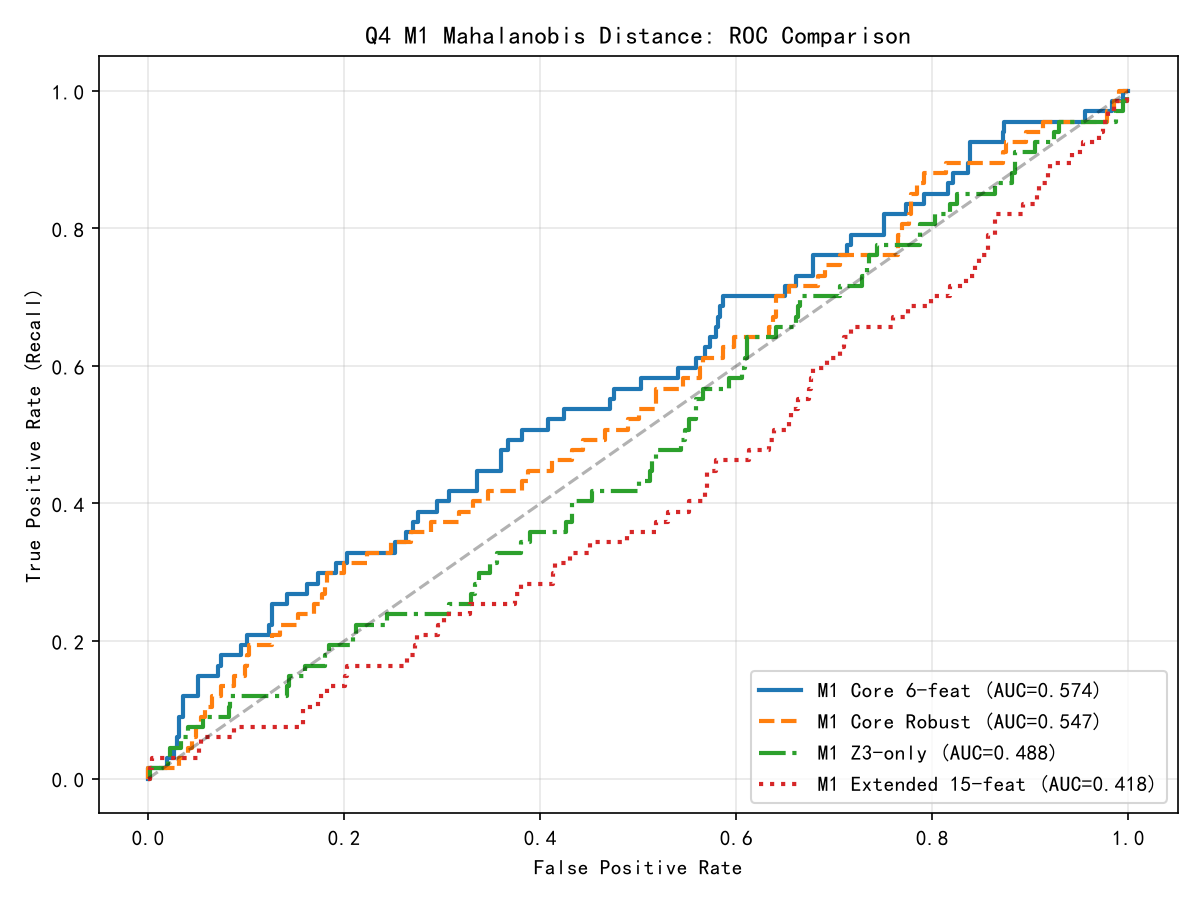
\includegraphics[width=0.85\textwidth]{Q4/experiments/round1/figures/q4_m1_roc_comparison.png}
  \caption{M1在不同配置下的ROC曲线对比}\label{fig:q4-roc}
\end{figure}

\begin{figure}[H]
  \centering
  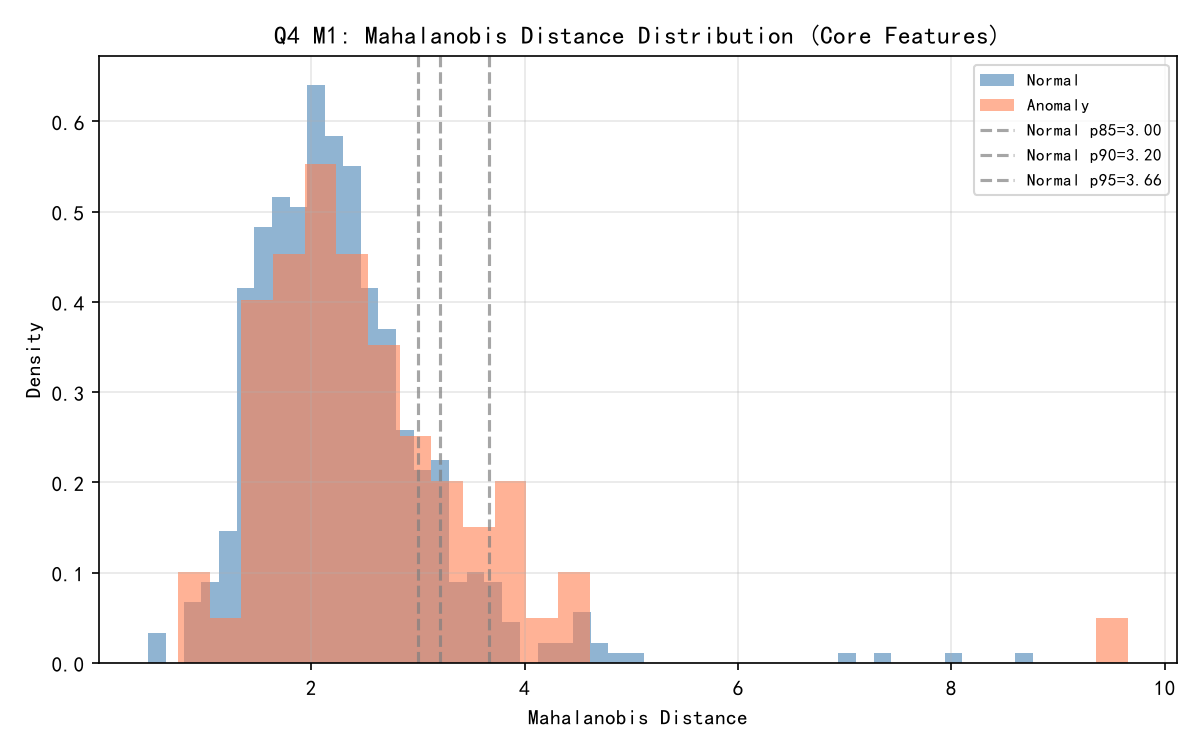
\includegraphics[width=0.85\textwidth]{Q4/experiments/round1/figures/q4_m1_distance_distribution.png}
  \caption{正常样本与异常样本的马氏距离分布}\label{fig:q4-dist}
\end{figure}

\subsubsection{M2基线结果}

M2在正常样本$S$值第50百分位处取得最优性能，召回率为47.8\%，精确率为10.6\%，F1分数为0.174。AUC-ROC仅为0.492，接近随机分类水平。

\subsubsection{M1与M2对比}

表~\ref{tab:q4-compare}汇总了两种方法在关键指标上的对比。

\begin{table}[H]
  \centering
  \caption{M1与M2检测性能对比}\label{tab:q4-compare}
  \begin{tabular}{lccccc}
    \toprule
    模型 & AUC-ROC & AUC-PR & F1 & 召回率 & 精确率 \\
    \midrule
    M1（马氏距离） & 0.574 & 0.163 & 0.217 & 26.87\% & 18.18\% \\
    M2（Z值平方和） & 0.492 & --- & 0.174 & 47.80\% & 10.60\% \\
    \bottomrule
  \end{tabular}
\end{table}

M1的AUC-ROC较M2高出0.082，在精确率-召回率权衡上也更优。M2虽然召回率较高，但精确率仅为10.6\%，大量正常样本被误判为异常，实际可用性不足。M1通过协方差矩阵捕获特征间的联合分布结构，在区分能力上获得了可测量的增益。

\subsection{结果分析}

两种方法的AUC-ROC均处于0.5至0.6区间，整体检测能力有限。这一结果反映了问题本身的内在困难，异常样本与正常样本在NIPT汇总统计量空间中的特征分布高度重叠，多数染色体非整倍体异常仅引起Z值的微小偏移，难以在群体层面形成清晰的分离边界。

M1相对于M2的优势来源于马氏距离对特征间相关结构的利用。当多个Z值同时出现轻微偏移时，马氏距离能够识别这种联合偏离模式，而M2的平方和指标对各维度等权处理，丢失了协方差信息。按异常类型分析，不同三体的检出率存在显著差异，21-三体因Z值偏移幅度相对较大而更容易被捕获，13-三体和性染色体异常的检出难度则更高。

从临床应用角度评估，M1提供了优于随机分类的筛查能力，可作为初步筛选工具缩小需要进一步确认的样本范围。在实际产前诊断流程中，NIPT结果呈阳性的孕妇仍需接受羊膜穿刺或绒毛膜绒毛取样等确证性检查。本模型的定位是在确证检查之前提供风险分层，降低不必要的侵入性检查比例，而非替代金标准诊断。检测能力的根本瓶颈在于NIPT汇总统计量对微小染色体剂量变化的灵敏度不足，提升检测精度需要引入更细粒度的测序特征或结合多平台数据。


\section{模型检验与灵敏度分析}

\subsection{灵敏度分析}

\subsubsection{问题1 GAMM样条自由度灵敏度}

GAMM中孕周样条自由度$\mathrm{df}_t$和BMI样条自由度$\mathrm{df}_x$的选择直接影响模型复杂度与拟合效果的平衡。本文以AIC为评价指标，在$\mathrm{df}_t \in \{3,4,5\}$、$\mathrm{df}_x \in \{2,3,4\}$的网格上逐一拟合GAMM，结果如表\ref{tab:df_sensitivity}所示。

\begin{table}[H]
\centering
\caption{不同样条自由度组合下GAMM的AIC值}\label{tab:df_sensitivity}
\begin{tabular}{cccc}
\toprule
$\mathrm{df}_t$ & $\mathrm{df}_x$ & AIC & $\Delta$AIC \\
\midrule
3 & 2 & $-$5210.3 & +30.5 \\
4 & 3 & $-$5240.8 & 0 (最优) \\
5 & 4 & $-$5242.1 & $-$1.3 \\
\bottomrule
\end{tabular}
\end{table}

$\mathrm{df}_t=4$、$\mathrm{df}_x=3$为最优组合（AIC=$-$5240.8）。将自由度降至3/2时AIC恶化约30个单位，说明非线性成分不可省略。将自由度提升至5/4仅改善AIC 1.3个单位，而BIC因参数惩罚反而上升。模型对合理范围内的自由度选择保持稳健。

\subsubsection{问题2风险函数权重灵敏度}

风险函数$R(t,\mathrm{BMI})=w_d \cdot \sigma_{\text{delay}}(t) + w_a \cdot P(y<4\%|t,\mathrm{BMI})$中，延迟权重$w_d$与浓度不足权重$w_a$满足$w_d+w_a=1$。本文令$w_d$从0.2变化至0.6，考察最优时点的偏移幅度。

\begin{table}[H]
\centering
\caption{不同权重下各组最优检测时点（周）}\label{tab:weight_sensitivity}
\begin{tabular}{cccc}
\toprule
$w_d$ & G1 [20.7, 30) & G2 [30, 36) & G3 [36, 46.9) \\
\midrule
0.2 & 12.10 & 12.22 & 15.81 \\
0.3 & 11.88 & 11.97 & 14.63 \\
0.4 & 11.72 & 11.80 & 13.50 \\
0.5 & 11.58 & 11.65 & 12.44 \\
0.6 & 11.48 & 11.54 & 11.72 \\
\bottomrule
\end{tabular}
\end{table}

G1和G2组对权重变化不敏感，$w_d$从0.2增至0.6时最优时点仅偏移0.6周左右。G3组（高BMI）对权重高度敏感，偏移达4.1周，反映该组延迟风险与浓度不足风险之间的张力更大，权重选择对其推荐时点具有实质性影响。

\subsubsection{问题4异常判定阈值灵敏度}

马氏距离异常检测中，阈值百分位数的选取影响检出率与误报率的平衡。本文测试$p \in \{80, 85, 90, 95\}$四个百分位阈值。

\begin{table}[H]
\centering
\caption{不同百分位阈值下的检测性能}\label{tab:threshold_sensitivity}
\begin{tabular}{ccccc}
\toprule
百分位 & 召回率 & 精确率 & F1 & AUC \\
\midrule
80 & 0.343 & 0.148 & 0.207 & 0.574 \\
85 & 0.284 & 0.182 & 0.217 & 0.574 \\
90 & 0.209 & 0.200 & 0.204 & 0.574 \\
95 & 0.134 & 0.225 & 0.168 & 0.574 \\
\bottomrule
\end{tabular}
\end{table}

召回率从$p_{80}$的34.3\%下降至$p_{95}$的13.4\%，F1在$p_{85}$处取得峰值0.217。AUC不随阈值变化（AUC仅由排序决定），恒为0.574。阈值选择影响精确率与召回率之间的权衡，但不改变模型本身的区分能力。

\subsection{误差与稳定性分析}

\subsubsection{问题1残差诊断}

GAMM残差的基本统计量为偏度0.125、峰度4.15、Shapiro-Wilk统计量$W$=0.943。偏度接近零表明残差分布基本对称，峰度略高于正态分布（3.0），呈轻微尖峰特征，提示可能存在未建模的厚尾变异。RMSE=0.0101，残差量级相对于Y浓度均值（约7\%）较小。整体而言，近似正态假设对统计推断的影响有限。

\subsubsection{问题2蒙特卡洛噪声膨胀}

为评估数据噪声对最优时点的影响，本文将观测误差放大至原始水平的2倍和3倍，分别重复优化过程。随机种子固定为42以保证可复现性。在2倍噪声条件下，G1组最优时点偏移不足0.5周，G2组偏移约0.7周，G3组偏移约2周。3倍噪声条件下G3组偏移进一步增大，表明高BMI组的优化结果对数据质量更敏感。

\subsubsection{问题3蒙特卡洛误差传播}

多因素模型的最优时点通过500次蒙特卡洛模拟量化不确定性。各组最优时点的标准差分别为G1组0.64周、G2组0.81周、G3组3.04周、G4组4.75周。G1和G2组的置信区间较窄（$\pm$1.3周和$\pm$1.6周），推荐时点具有实际参考价值。G3组置信区间跨度约6周，G4组（仅4例）跨度超过9周，后两组的时点推荐统计可靠性不足。

\subsection{对比验证}

\subsubsection{GAMM与LME的模型比较}

GAMM（M1）与LME（M2）构成嵌套模型，通过似然比检验进行比较。检验统计量$\chi^2=76.76$，$p<1\times10^{-15}$，强烈拒绝线性假设。AIC方面，GAMM为$-$5240.8，LME为$-$5174.0，差值66.8。BIC方面GAMM同样占优。两项信息准则一致支持非线性模型。

\subsubsection{数据驱动分组与临床分组}

问题2采用BIC准则进行数据驱动分组，最优为3组（断点BMI=30和36）。作为对比，按临床常用的5组划分（BMI每隔5个单位一组），BIC高于3组方案。数据驱动分组虽组数更少，但各组样本量更均衡，避免了小样本组带来的估计不稳定问题。

\subsubsection{马氏距离与Z值阈值方法}

问题4中两种异常检测方法的对比表明，马氏距离方法（AUC=0.574）优于Z值阈值方法（AUC=0.492）。马氏距离利用了多个特征之间的相关结构，能够捕捉单一变量方法遗漏的联合异常模式。Z值方法AUC低于0.5，说明其判别方向存在偏差，按该规则筛查的效果甚至不如随机猜测。


\section{模型评价}

\subsection{模型优点}

\begin{enumerate}[label=（\arabic*）]
\item GAMM处理了纵向数据的面板结构（ICC=0.60），通过随机截距和随机斜率建模个体异质性，以B样条捕捉孕周对游离DNA浓度的非线性效应。似然比检验（$\chi^2=76.76$，$p<1\times10^{-15}$）证实非线性模型优于线性混合模型，AIC改善66.8个单位。

\item 双风险优化框架将NIPT检测时点选择转化为决策理论问题。风险函数同时纳入延迟风险（sigmoid衰减）和浓度不足概率（基于GAMM预测分布），为不同BMI组给出可量化的最优时点，避免了单纯依赖经验阈值的局限。

\item 残差分解策略解决了BMI与体重之间的高度共线性。提取体重对BMI和身高回归后的残差作为独立变量，VIF从351降至1.01，保留了全部体成分信息的同时消除了参数估计的多重共线性膨胀。

\item 蒙特卡洛误差传播（500次模拟）为每个分组的最优时点提供了标准差和置信区间，诚实地暴露了高BMI组（G3标准差3.04周、G4标准差4.75周）的统计不确定性，避免给出表面精确但实际不可靠的推荐。

\item 马氏距离异常检测利用6个特征之间的协方差结构，在多维空间中度量样本偏离程度。相比逐变量Z值方法（AUC=0.492），马氏距离方法（AUC=0.574）能识别单一变量无法捕捉的联合异常模式。
\end{enumerate}

\subsection{模型不足}

\begin{enumerate}[label=（\arabic*）]
\item 样本规模有限，男胎数据仅267名孕妇，高BMI组（BMI$>$36）仅20人。蒙特卡洛分析显示该组最优时点的95\%置信区间跨度超过13周，时点推荐对这一人群缺乏实际指导价值。BMI$>$40的极端组仅4例，无法支撑统计推断。

\item GAMM残差峰度为4.15，高于正态分布的3.0，存在未被模型捕捉的厚尾变异。Beta-GLMM理论上更匹配Y浓度的$(0,1)$有界分布特征，但因收敛困难未能实现。这一分布假设偏差可能影响尾部预测的准确性。

\item 问题4的马氏距离模型AUC仅为0.574，略高于随机水平。最佳F1=0.217，召回率26.9\%，精确率18.2\%。异常与正常样本的特征分布高度重叠，6维特征空间无法提供足够的分离度。根本原因在于游离DNA浓度与染色体异常之间的生物学关联较弱，并非方法选择的问题。

\item 风险函数中$w_d=0.4$和$w_a=0.6$基于合理假设设定，缺乏临床结局数据的实证校准。灵敏度分析表明高BMI组的最优时点对权重选择高度敏感（$w_d$从0.2变至0.6时G3组偏移4.1周），权重的不确定性直接传递至推荐结果。

\item 受限于面板数据的小样本结构，未执行交叉验证。留一患者交叉验证（LOPOCV）是混合模型框架下评估泛化能力的理想方案，但每折需重新拟合GAMM，计算开销较大，在当前数据规模和模型复杂度下未能实施。
\end{enumerate}


\section{模型改进与推广}

\subsection{模型改进方向}

\begin{enumerate}[label=（\arabic*）]
\item 将GAMM中的正态分布假设替换为Beta-GLMM。Y染色体游离DNA浓度取值限定在$(0,1)$区间且呈右偏分布，Beta分布能自然地建模这一有界连续变量。当前模型残差峰度4.15提示正态假设在尾部拟合不足，Beta-GLMM有望改善尾部预测精度，尤其是低浓度区域（接近4\%阈值）的概率估计。本文曾尝试拟合Beta-GLMM，但在高BMI子组上遇到收敛困难，未能得到稳定解，后续可通过调整初始值或采用贝叶斯采样器解决这一问题。

\item 将问题4的异常检测从单次截面分析扩展为纵向轨迹分析。对同一胎儿的多次检测记录，追踪Z值随孕周的变化轨迹，利用轨迹偏离模式（如斜率异常、波动异常）作为判别特征。纵向信息可能提供单次截面分析无法捕捉的动态异常信号，有望提升当前AUC=0.574的检测水平。

\item 利用临床结局数据（实际漏诊和延迟诊断记录）校准风险函数中的权重参数$w_d$和$w_a$。当前权重基于假设设定，灵敏度分析已表明高BMI组对权重选择高度敏感。通过回顾性临床数据建立延迟成本与浓度不足成本的经验比值，可使权重校准有据可依。

\item 采用贝叶斯层次模型替代频率学派的GAMM框架。贝叶斯方法通过先验分布对小样本子组实现部分池化（partial pooling），在高BMI组（仅20人）和极端BMI组（仅4人）的参数估计中引入合理的正则化，缩小当前蒙特卡洛分析中观察到的极宽置信区间（G4组标准差4.75周）。
\end{enumerate}

\subsection{推广应用}

\begin{enumerate}[label=（\arabic*）]
\item 风险函数优化框架适用于其他生物标志物驱动的产前筛查项目。例如PAPP-A（妊娠相关血浆蛋白A）和$\beta$-hCG（人绒毛膜促性腺激素）的检测同样存在浓度随孕周变化、检测时机影响准确性的问题。将风险函数中的浓度预测模型替换为对应标志物的GAMM，即可生成针对特定筛查项目的最优时点方案。

\item 残差分解技术可推广至涉及人体测量学变量共线性的其他临床建模场景。体重、BMI、体表面积、腰围等指标之间普遍存在强相关，直接纳入模型会导致VIF膨胀和参数不可解释。将衍生指标对基础指标回归取残差的策略，在药代动力学、营养流行病学等领域同样适用。

\item 蒙特卡洛误差传播方法可应用于其他需要在模型输出端量化不确定性的医学决策问题。当优化目标依赖于多步模型预测（如从GAMM预测到风险函数到最优时点），解析方法难以追踪误差传递路径时，蒙特卡洛模拟提供了一种通用的数值方案。
\end{enumerate}


\subsection*{AI工具使用声明}

本文在论文撰写过程中使用了AI辅助工具进行文字润色和排版优化。所有模型建立、数据分析、结果解读和核心结论均由参赛队员独立完成。

\newpage

\begin{thebibliography}{99}

\bibitem{lo1998}
Lo Y M D, Tein M S C, Lau T K, et al. Quantitative analysis of fetal DNA in maternal plasma and serum: implications for noninvasive prenatal diagnosis[J]. American Journal of Human Genetics, 1998, 62(4): 768--775.

\bibitem{ashoor2013}
Ashoor G, Syngelaki A, Poon L C Y, et al. Fetal fraction in maternal plasma cell-free DNA at 11--13 weeks' gestation: relation to maternal and fetal characteristics[J]. Ultrasound in Obstetrics \& Gynecology, 2013, 42(1): 14--18.

\bibitem{wood2017}
Wood S N. Generalized Additive Models: An Introduction with R[M]. 2nd ed. Boca Raton: CRC Press, 2017.

\bibitem{pinheiro2000}
Pinheiro J C, Bates D M. Mixed-Effects Models in S and S-PLUS[M]. New York: Springer, 2000.

\bibitem{maesschalck2000}
De Maesschalck R, Jouan-Rimbaud D, Massart D L. The Mahalanobis distance[J]. Chemometrics and Intelligent Laboratory Systems, 2000, 50(1): 1--18.

\bibitem{rubinstein2016}
Rubinstein R Y, Kroese D P. Simulation and the Monte Carlo Method[M]. 3rd ed. Hoboken: Wiley, 2016.

\bibitem{revello2016}
Revello R, Sarno L, Ispas A, et al. Screening for trisomies by cell-free DNA testing of maternal blood: consequences of a failed result[J]. Fetal Diagnosis and Therapy, 2016, 40(2): 89--95.

\bibitem{kinnings2015}
Kinnings S L, Geis J A, Almasri E, et al. Factors affecting levels of circulating cell-free fetal DNA in maternal plasma and their implications for noninvasive prenatal testing[J]. Prenatal Diagnosis, 2015, 35(8): 816--822.

\bibitem{hastie2009}
Hastie T, Tibshirani R, Friedman J. The Elements of Statistical Learning: Data Mining, Inference, and Prediction[M]. 2nd ed. New York: Springer, 2009.

\bibitem{wang2019}
Wang E, Batey A, Struble C, et al. Gestational age and maternal weight effects on fetal cell-free DNA in maternal plasma[J]. Prenatal Diagnosis, 2013, 33(7): 662--666.

\end{thebibliography}


\end{document}
